%\begin{wraptable}[6]{r}{0.56\textwidth}
%\vspace{-0.8cm}
%\centering{
%  \begin{tabular}{|l|r|r|p{0.1\textwidth}|}
%    \hline
%          & HAP                     & experiment          & ref.\\
%    \hline 
%    $\KB$ & $11 \pm 2.5$ \kBT       & 10 \kBT               & \cite{Naetal15,VeBrPa15,NAGLE2000159,PhysRevLett.113.248102}\\
%    \hline 
%    $\KA$ & $34$ \kBT \; nm$^{-2}$  & 30--40 \kBT nm$^{-2}$ & \cite{Nagle17, Nagle17-2}\\
%    \hline 
%    $\KTH$ & $12$ \kBT \; nm$^{-2}$ & 10 \kBT nm$^{-2}$     & \cite{KUZMIN2005, KoNa15} \\ \hline
%  \end{tabular}
%}
%  \vspace{-8pt}
%\caption{\label{tab:moduli} \footnotesize Comparison of values of elastic
%  moduli from the experimental literature and derived by HAP
%  simulation.} 
%\end{wraptable}


\section{Preliminary work}
\label{sec:preliminary_work}


%While the results show great promise in the field of collective body
%hydrodynamics, several outstanding issues need to be addressed. These
%include a thorough analysis of elastic properties of our coarse-grained
%bilayers and efficiently simulating three-dimensional collective
%hydrodynamics of amphiphilic particles.
%We must also incorporate electric charge and account
%for how external fields control particle self-assembly.


%
%The HAP project was initiated in 2017 by PI RR and YNY. The lead author
%on our first paper~\cite{Fu2018_SIAM} was Szu-Pei Fu, who was PI YNY's
%PhD student and is currently a postdoc with PI RR. The collaboration
%involved theoretical work and simulation. The theoretical work included
%model development, proving the first variation formula~\eqref{stress}
%and force-free law, and an energy-based uniqueness theorem for the
%exterior domain problem~\eqref{SL}. 
%Coauthors Andreas Kl\"ockner
%(Computer Science, UIUC, NSF CAREER \#1654756) and his PhD student Matt
%Wala provided their Quadrature by Expansion, or QBX algorithm and Fu ran
%simulations on NJIT clusters.
%
%\begin{wraptable}[11]{l}{0.43\textwidth}
%\centering{
%  \begin{tabular}{|l|l|l|l|}
%    $n$   & (rel.~err.)$_F$
%    &  (rel.~err.)$_G$ \\
%    \hline
%% 32   &   4.07466     &   1.56437\\
%% 64   &   0.24664     &   0.03476\\
%% 128  &   0.00063     &   0.00006\\
%  32  & $4.07 \times 10^{+0}$ & $1.56 \times 10^{+0}$ \\
%  64  & $2.47 \times 10^{-1}$ & $3.48 \times 10^{-2}$ \\
%  128 & $6.30 \times 10^{-4}$ & $6.00 \times 10^{-5}$ 
%  \end{tabular}}
%\vspace{-5pt}
%\caption{\label{tab:spectral_force} 
%\footnotesize  Relative numerical errors (rel.~err.)$_F = \max_{i}
%  \|\mathbf{F}_i-\mathbf{F}_i^{\text{exact}}\|/\|\mathbf{F}_i^{\text{exact}}\|$
%  and (rel.~err.)$_G = \max_{i}
%  \|\mathbf{G}_i-\mathbf{G}_i^{\text{exact}}\|/\|\mathbf{G}_i^{\text{exact}}\|$
%  for force and torque respectively as a function of number of grid
%  points $n$ per particle.  The data is for $N = 5$ particles; two of
%  the particles are nearly touching at a distance 1\% of particle
%  diameter.} 
%\end{wraptable}
\begin{wrapfigure}[11]{r}{0.5\textwidth}
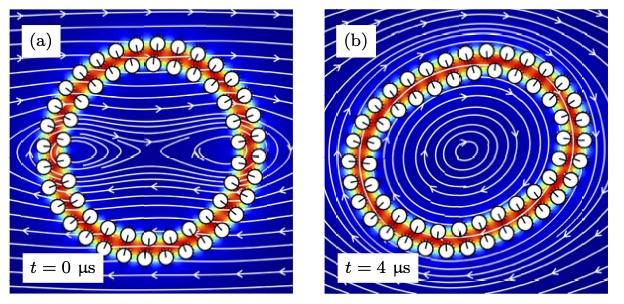
\includegraphics[width=0.5\textwidth]{figures/TankTreading.jpg}
\caption{\label{fig:JPv_linearshear}The JP vesicles undergo tank-treading in background shear flow.}
\end{wrapfigure}
PIs RR and YNY started work on HAP modeling with Szu-Pei Fu (then PI
YNY's student and now PI RR's postdoc) and collaborators in 2017. The
interactions between Janus particles (JPs) were formulated as a
second-kind integral equation, which is coupled to the Stokes equations
for the surrounding incompressible fluid at the zero-Reynolds-number
limit. Numerical simulations of a JP suspension revealed self-assembly
of JPs into micelles, bilayers, and vesicles (self-enclosing bilayers),
providing an alternative means for computing mechanical moduli, which
often requires the knowledge of an equation of state from experiments on
a colloidal membrane~\cite{Balchunas2019_SM}.

\begin{wrapfigure}[14]{l}{0.475\textwidth}
%\vspace{-10pt}
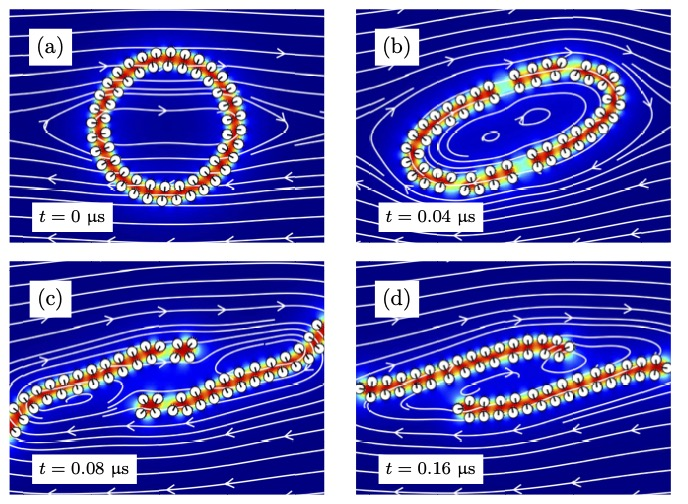
\includegraphics[width=0.475\textwidth]{figures/Rupture.jpg}
\caption{\label{fig:JPv_rupture}The JP vesicles rupture under large shear rates.}
\end{wrapfigure}
%
The results in~\cite{Fu2018_SIAM}
successfully demonstrated gradient-driven
self-assembly of amphiphilic particles into two-dimensional micelles and
bilayer membranes with realistic values of the model parameters
for decay
length %$\rho=2.5$~nm
(based on measurements of hydrophobic attraction
between surfactant-coated surfaces~\cite{ErLjCl89, Lin2005,
  Parsegian, Israelachvili80}), particle diameter %$\delta = 2.0$~nm
(the
physical monolayer thickness~\cite{Boal}), and interfacial tension
%$\gamma = 4$~pN nm$^{-1}$
(based on measurements for single-component
bilayer lipid membranes~\cite{GarciaSaez, KUZMIN2005, Petelska2012,
Jackson2016}).
%
%\begin{wraptable}[10]{l}{0.43\textwidth}
%  \vspace{-6pt}
%\centering{
%  \begin{tabular}{|l|l|l|l|}
%    $n$   & (rel.~err.)$_F$
%    &  (rel.~err.)$_G$ \\
%    \hline
% 32   &   4.07466     &   1.56437\\
% 64   &   0.24664     &   0.03476\\
% 128  &   0.00063     &   0.00006\\
%  32  & $4.07 \times 10^{+0}$ & $1.56 \times 10^{+0}$ \\
%  64  & $2.47 \times 10^{-1}$ & $3.48 \times 10^{-2}$ \\
%  128 & $6.30 \times 10^{-4}$ & $6.00 \times 10^{-5}$ 
%  \end{tabular}}
%\vspace{-8pt}
%\caption{\label{tab:spectral_force} 
%\footnotesize  Relative numerical errors (rel.~err.)$_F = \max_{i}
%  \|\mathbf{F}_i-\mathbf{F}_i^{\text{exact}}\|/\|\mathbf{F}_i^{\text{exact}}\|$
%  and (rel.~err.)$_G = \max_{i}
%  \|\mathbf{G}_i-\mathbf{G}_i^{\text{exact}}\|/\|\mathbf{G}_i^{\text{exact}}\|$
%  for force and torque, respectively, as a function of number of grid
%  points $n$ per particle. The data is for $N = 5$ particles; two of the
%  particles are nearly touching at a distance of 1\% of the particle
%  diameter.} 
%\end{wraptable}
%
Results in this work show great potential to study Janus
colloids~\cite{Bradley2017,Mallory2017} and the morphology of colloid
surfactants~\cite{Bradley2016}.  For example, with the flexibility of
the model, we can specify the boundary condition on JP surfaces based on
the chemicals used in experiments.

%The paper \cite{Fu2018_SIAM} considered three types of simulations.
%The first measured bending by
%loading a partially clamped planar bilayer. The second used a harmonic
%bond to dilate a circular bilayer. The third measured tilt using a decay
%equation from~\cite{KUZMIN2005}. These simulations isolated three of the
%five deformations of~\eqref{ansatz3}, enabling us to read off elastic
%moduli from simulation data. The results agreed remarkably well with the
%values reported in the experimental literature.% (Table~\ref{tab:moduli}).
%The agreement is underscored by the fact that the two main HAP
%parameters, $\gamma$ and $\rho$, were assigned physical values from the
%outset rather than being tuned to fit data. 



%
%This study presents a coarse-grained model for JP vesicles that focuses
%on the hydrophobic interactions between coarse-grained lipids and
%hydrodynamic interactions. In contrast to molecular dynamic simulations,
%the hydrophobic interactions exhibit the self-assembly property of the
%lipid bilayer membrane. The proposed energy potential combined with the
%mobility problem for rigid body motions captures membrane mechanics
%including deformations, stretching modulus, and permeability of a JP
%membrane. 
%

%
%This work is highly applicable with fields in material science
%and condensed matter physics such as Janus
%colloids~(\cite{Bradley2017,Mallory2017}) and the setup can be tuned to
%match experimental results such as the morphology of colloid
%surfactants~(\cite{Bradley2016}). 
%%

%This can be an assist to study of interparticle interactions and chemical compositions in industry.

%Integral equation methods are used to solve the mobility problem and the
%previously introduced HAP model. We describe a method to calculate the
%hydrophobic forces and torques on each individual rigid body that avoids
%singular integrals. In addition to the HAP forces and torques, we use a
%short-range repulsion to avoid unphysical contact. 


PIs RR, BQ, and YNY initiated a collaboration in summer 2020 to study
the hydrodynamics of JP suspensions. They used the integral formulation
in~\cite{Fu2018_SIAM} and an improved numerical algorithm to simulate
the hydrodynamics of JP vesicles in background flows. Under a linear
shear flow (Figure~\ref{fig:JPv_linearshear}), JP vesicles exhibited
elongation and tank-treading dynamics observed for a lipid bilayer GUV.
The total length of a JP vesicle was conserved and the decay rate of the
reduced area was independent of the shear rate.  Moreover, the model
described membrane rupture in high shear rates
(Figure~\ref{fig:JPv_rupture}). Therefore, the method can be applied to
vesicles undergoing topological changes which is difficult to simulate
when using a continuum model that represents vesicles as closed and
continuous curves.

\begin{wrapfigure}[11]{l}{0.6\textwidth}
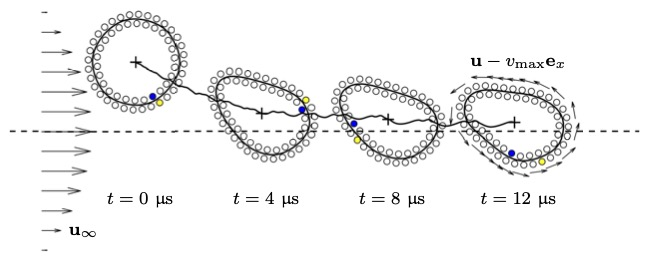
\includegraphics[width=0.6\textwidth]{figures/Slipper.jpg}
\caption{\label{fig:JP_poiseuille}The JP vesicle takes on the asymmetric
  slipper shape in parabolic flow.}
\end{wrapfigure}
The PIs used the simulation data to estimate the inter-monolayer
friction, membrane permeability constant, and the membrane
stretching modulus~\cite{chabanon2017, sch_vla_mik2010}. The range
of friction coefficients agree with values reported
by~\cite{denOtter2007,WuoEd06} in their molecular dynamics study. The
coarse-graining level of the JP vesicle has a larger length scale than
molecular dynamics simulations, and we are now conducting convergence
studies to investigate how physical properties of the assembly like the
friction coefficient and membrane permeability depend on the JP particle
shape and size.

The study also simulated the spatial migration of a JP vesicle in a
parabolic shear flow (Figure~\ref{fig:JP_poiseuille}). Replicating the
hydrodynamics of a GUV in a Poiseuille flow~\cite{Kaoui09,
dan_vla_mis2009, cou_kao_pod_mis2008}, the JP vesicle moves toward the
center of the shear flow, and has a slight decrease in reduced area.
For the parameters we used in the simulation, the JP vesicle takes on an
asymmetric, ``slipper" shape as it settles above the centre of flow and
exhibits tank-treading motion. A qualitative agreement is made by
comparing the JP vesicle shape with the two-dimensional inextensible
membrane in continuum modeling simulations~\cite{Kaoui09,
dan_vla_mis2009, cou_kao_pod_mis2008}. An interesting result contrast
with continuum results is that the JP vesicle oscillates at a height
slightly above the centre of the Poiseuille flow. 

%The single JP vesicle simulations end with obtaining JP bilayer stretching 
%modulus $K_A$ and hydraulic permeability constant $P$. We extract these 
%physical quantities from the Laplace pressure relationship that $R\Delta P$ is 
%proportional to JP bilayer stretch. We describe the aqueous flux in membrane 
%using a differential equation~\ref{eq:perm} and solve for the theoretical 
%permeability constant $P$. In spite of producing these values with some discrepancy
%using the default parameter set, we provide a new framework in measuring coarse-grained 
%membrane permeability.


\begin{wrapfigure}[15]{l}{0.5\textwidth}
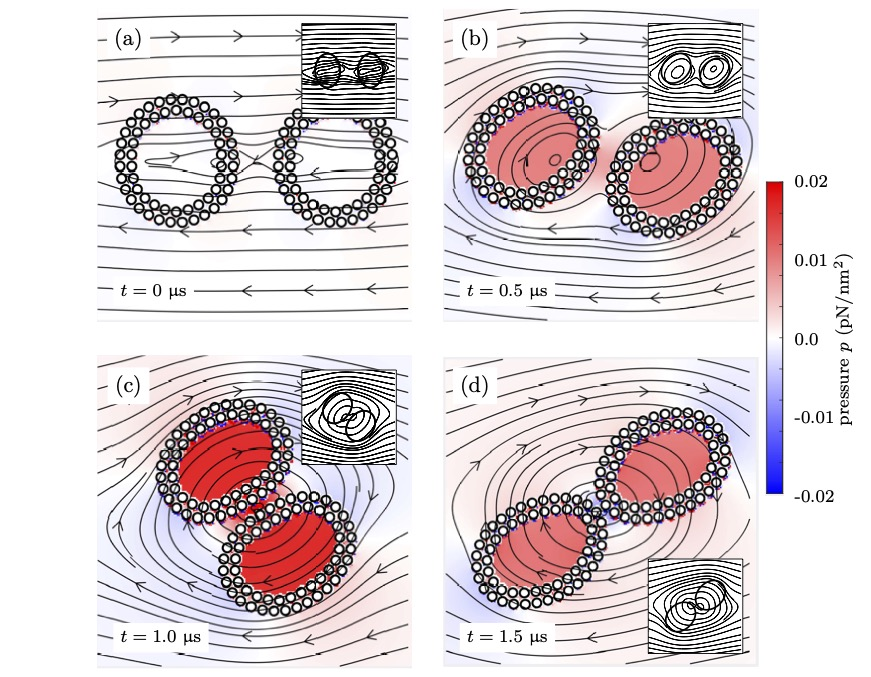
\includegraphics[width=0.5\textwidth]{figures/ShearDoublet.jpg}
\caption{\label{fig:JPv_interactions} Vesicle-vesicle interaction for JP
  vesicles in shear flow.}
\end{wrapfigure}
The PIs further simulated the hydrodynamics interactions between two JP
vesicles (Figure~\ref{fig:JPv_interactions}), and drew comparisons with
simulation results of two vesicles described by the Helfrich continuum
model. A comparison of the vesicle shapes and the streamlines
demonstrate remarkable similarities. The two overlapping trajectories of
the JP vesicles' centroids in a shear flow evolve as expected when the
two centroids are initialized on the same horizontal level. The PI
observed a rotating behaviour that is observed for models involving
vesicle adhesion~\cite{qua-vee-you2019, abb-far-ezz-ben-mis2021}. The
hydrophobic attraction led to this adhesive effect when two JP bilayers
are sufficiently close. We also performed simulations of a pair
of JP vesicles suspended in an extensional flow (see \cite{FuQuRyYo22}).
%By varying the initial
%vertical displacement of the vesicles' centroids, we can control for
%divergent trajectories and obtain similar results to the continuum
%model.

One of the main mathematical innovations in the PIs collaboration is a
novel alternative integral form for calculating the force and torque
that avoids singular integral evaluation. These alternative integrals
allow the accurate resolution of trajectories over long times without
having to rely on computationally expensive quadratures. Future goals
include extending the current framework to a three-dimensional JP
vesicle system. This will require additional algorithmic implementation
including a fast summation method such as the fast multipole method \cite{Yan2019}.



